\documentclass[letterpaper,12pt]{article}

%\usepackage[hypertex]{hyperref}
\usepackage{comment}
\RequirePackage{GE05}
% this inputs graphicx, too

\newcommand{\GDP}{\mbox{\em GDP\/}}
\newcommand{\NDP}{\mbox{\em NDP\/}}
\newcommand{\GNP}{\mbox{\em GNP\/}}
\newcommand{\NX}{\mbox{\em NX\/}}
\newcommand{\NY}{\mbox{\em NY\/}}
\newcommand{\CA}{\mbox{\em CA\/}}
\newcommand{\NFA}{\mbox{\em NFA\/}}
\newcommand{\Def}{\mbox{\em Def\/}}
\newcommand{\CPI}{\mbox{\em CPI\/}}
\newcommand{\phm}{\phantom{--}}

\def\ClassName{The Global Economy}
\def\Category{Professor David Backus}
\def\HeadName{Final Exam}

\begin{document}
\parindent = 0.0in
\parskip = \bigskipamount
\thispagestyle{empty}%
\Head

\centerline{\large \bf \HeadName}%
\centerline{Revised:  \today}

\bigskip
You have 100 minutes to complete this exam.  Please answer each question in the space provided.
You may consult one page of notes and a calculator, but devices capable of wireless transmission
are prohibited.

I understand that the honor code applies: I will not lie, cheat, or
steal to gain an academic advantage, or tolerate those who do.

\begin{flushright}
\rule{4in}{0.5pt} \\ (Name, section, and signature)
\end{flushright}

\begin{figure}[h]
    \centering
    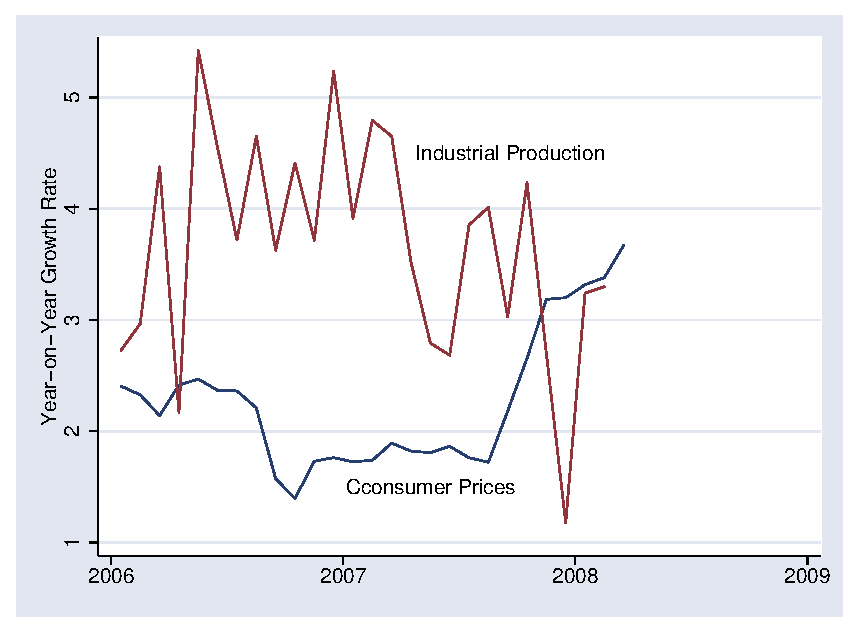
\includegraphics[scale=0.8]{final_08.eps}
    \caption{Growth in prices and industrial production in the 
    Euro Zone.} 
    \label{fig:ez}
\end{figure}

\begin{enumerate}
% ---------------------------------------------------------
\item {\it Supply and demand in the Euro Zone (30 points).\/}
As the CFO of Heineken International, you are considering
the likely evolution of interest rates in the Euro Zone.  
You quickly run through the following questions:  
%
\begin{enumerate}

\item Over the 2-year period as a whole, 
    what has happened to inflation and output?  
    See Figure \ref{fig:ez}; 
    nothing is needed beyond what you see there.
    (5~points)

\item In the aggregate supply and demand framework, 
    do you think the movements in prices and output 
    you mentioned above suggest a shift in supply or demand?  Why?  
    In principle, 
    how should the European Central Bank respond to such a shift? 
    (15~points) 

\item How do you think the European Central Bank is 
likely to respond?
How do you see short-term Euro Zone 
interest rates moving over the next 12 months? Why?  
(10~points) 

\end{enumerate}

%\begin{comment}
Answer.
\begin{enumerate}
\item Inflation is up sharply, output is flat to down. 

\item The combination in (a) suggests a shift up/left in supply.
Why?  Because output and inflation have moved in opposite directions.
Since supply shocks should be accommodated/reinforced, 
the ECB should raise the short-term interest rate.

Grading:  10 for noting shift in supply, 
5 for the comment about policy.  

\item The ECB's primary mission is stable prices, 
so you should see an increase in interest rates.
This could also be expressed in terms of a Taylor rule, 
possibly with a larger coefficient on inflation 
than output growth.  

\end{enumerate}
%\end{comment}


%\pagebreak \phantom{bla} \pagebreak %\phantom{bla} \pagebreak
% ---------------------------------------------------------
\item {\it Risk and reward in Romania (30 points).\/} 
Romania has had a chaotic history since unification 
under the Ottoman Empire in 1859 and independence in 1878.
In 1940, it lost territory to Hungary and the Soviet Union; 
after World War II, the remainder became part of the Soviet bloc.  
Since December 1989, when the communist regime fell, 
Romania has embarked on a cautious path of reform 
and has been an official member of the European Union since January 2007.
Romania remains a poor country, 
with GDP per capita below Poland and Hungary 
but above Bulgaria and Serbia.  
The current minority government, which faces an election in November, 
has been notably slow to accelerate reform, 
failing specifically to address concerns expressed by the EU and IMF 
about fiscal policy, the current account, judicial reform, and corruption. 
Current economic indicators include:
%
%\tabcolsep=0.25in
\begin{center}
\begin{tabular}{lcr}
  {\it Indicator}   &&  {\it Value}     \\
  GDP growth (real) &&  6\%       \\
  Inflation         &&  5\%       \\
  Short-term interest rate &&  8\%   \\
  Fiscal balance:  total  (ratio to GDP)    &&  --2.6\%  \\
  Fiscal balance:  primary  (ratio to GDP)  &&  --0.7\%   \\
  Government debt (ratio to GDP)            &&  18\%       \\
  Current account balance (ratio to GDP)    &&  --11.3\%   \\
  Current account balance (US dollars) &&   --23b   \\
  Net foreign assets (ratio to GDP)         &&   --19\%   \\
  Foreign reserves (US dollars)           &&  39b  \\
\end{tabular}
\end{center}
%
Text and numbers adapted from Economist Intelligence Unit, 
{\it Country Profile\/} and {\it Country Risk Service\/}.  
%Variables marked by * are ratios to GDP (nominal to nominal).  

\begin{enumerate}

\item Why do the primary and total fiscal balances differ?  
(5~points)

\item How do you see the government debt evolving over the next year?  (10~points)

\item In 2007, the capital inflow implied by the current account deficit consisted of roughly  equal parts
    direct investment, foreign loans to banks, and foreign loans to 
    other sectors.  Some of the foreign loans were said to be 
    denominated in foreign currency.
    Given this information and the numbers above, 
    does the current account deficit concern you?  
    Why or why not?  
    (10~points)

\item Overall, what do you see as the major risks to a short-term investor in government or private sector debt?  
    Would you recommend such an investment?  Why or why not?  
    (5~points) 
\end{enumerate}

%\begin{comment}
Answer.
\begin{enumerate}
\item The difference is interest payments on government debt:
the total balance includes them as an expenditure, 
the primary balance does not.  

\item Debt dynamics work like this:  
\[
    \frac{\mbox{\em B}_{t+1}}{Y_{t+1}} \;=\; 
            \left( \frac{1+i}{1+g} \right)
            \frac{\mbox{\em B}_{t}}{Y_{t}} + (1+g)^{-1} 
            \frac{\mbox{\em D}_{t}}{Y_{t}} .
\]
With $ i = 8\%$ and $ g = 6 + 5 = 11\%$, 
the numbers tell us that next year's ratio of government debt ($B$) 
to GDP ($Y$) will rise slightly:
\[
    (1.08/1.11) \times 0.18 + (1.11)^{-1} \times 0.007 \;=\; 0.181 .
\]
That is:  next year's debt to GDP ratio will be 18.1\%, 
up from 18\% this year --- itself a modest number.
In short, there's no sign here of it exploding.  
There are two reasons for this:  the primary deficit is modest
and the (nominal) growth rate exceeds the interest rate.  


Grading:  10 points for something like this analysis.  

\item These numbers are bigger, the question is whether 
they concern you or not.
You could (but need not) start with
 a similar analysis of net foreign assets;
you're missing net exports, but could either estimate that from 
net foreign assets and the interest rate or simply plug
in the current account as a rough guess.  
If you do the latter, you get 
\begin{eqnarray*}
    \frac{\mbox{\em NFA}_{t+1}}{Y_{t+1}} &=& 
            \left( \frac{1+i}{1+g} \right)
            \frac{\mbox{\em NFA}_{t}}{Y_{t}} + (1+g)^{-1} 
            \frac{\mbox{\em NX}_{t}}{Y_{t}} \\
           &=& (1.08/1.11) \times (-0.19) + (1.11)^{-1}\times(-0.113)
               \;=\; -0.287 .
\end{eqnarray*}
In short, there's a substantial decrease in net foreign assets.
The level, however, remains small:  
lots of countries have more foreign liabilities than this.  

Is this a problem?  
It depends!  
On what?  On what the funds are invested in.  
Lawson's doctrine is a good starting point:  
that private flows aren't a concern.
And since we've seen the government deficit is much smaller
than the government deficit, most of this must be private.
A counterargument is that the debt component could cause problems
anyway, esp loans to banks, which might be seen as implicitly 
backed by the government. 
Another possible concern is the foreign denomination:
a fall in the value of the currency could make these much 
more expensive to pay back.  
The large quantity of reserves gives you some protection 
against this. 
Direct investment is of less concern, since it's not a debt 
claim:  if the economy does poorly, 
the value of the claim should adjust.  

Grading:  full points for either the calculation 
or the discussion.  

\item 
My sense (and this is not required of your answer) is that 
the institutions of the EU make it unlikely Romania 
will default, but there remains a modest chance of a dramatic fall 
in the value of the currency.  



\end{enumerate}
%\end{comment}


%\pagebreak \phantom{bla} \pagebreak \phantom{bla} \pagebreak
% ---------------------------------------------------------
\item {\it Miscellany (40 points).}
%
\begin{enumerate} 

\item {\it Foreign exchange market intervention.\/}
Use a hypothetical central bank balance sheet to show how
purchases of foreign currency affect the bank's assets and liabilities. What does this purchase do to the supply of money (currency)? 
(10~points)

\item {\it Housing starts.\/}
Make the case that housing starts is a 
leading indicator of economic activity in the US.  Be specific.  
(10~points)

\item {\it Price of the euro.\/}
Right now, the euro is ``overvalued'' in PPP terms relative to the
dollar (goods are more expensive in Europe) and Euro Zone short-term interest rates remain 2-3\% above US interest rates.
Given these facts, how would you expect the euro/dollar exchange rate to change over the next 6 months?  6 years?
How good is each of these informed guesses?  
(10~points)


\item {\it Zimbabwe.\/}
Summarize the chain of circumstances that produced 
hyperinflation in Zimbabwe.
In your view, what steps are needed to break the chain?  
(10~points)


\end{enumerate}

%\begin{comment}
Answers.
\begin{enumerate}
\item Foreign exchange intervention works like this.  If a central bank buys foreign currency, it collects foreign currency and 
    issues domestic currency in return. 
    The latter is an increase in the domestic money supply.   
    Suppose, for example, the central bank
     starts with the balance sheet
    %
\begin{center}
\begin{tabular}{lrclr}
               Assets  &     &&     Liabilities                     \\  
               \hline 
               FX Reserves &  100 &&     Monetary Base &  200   \\    
               Bonds   & 100 && \\
\end{tabular}
\end{center}
%
The purchase of 25 worth of foreign currency 
changes the balance sheet to
%
\begin{center}
\begin{tabular}{lrclr}
               Assets  &     &&     Liabilities                     \\ 
               \hline 
               FX Reserves &  125 &&     Monetary Base &  225   \\    
               Bonds   & 100 && \\
\end{tabular}
\end{center}
%
Grading:  10 points for similar description of 
how balance sheet changes.
    
\item The easiest way is to calculate the cross-correlation function
for housing starts and a measure of economic activity --- say
industrial production.
Since (the growth rate of) housing starts is strongly    
correlated with future industrial production (also growth), 
then it's  a leading indicator.  

Grading:  10 points for something like this.  

\item  Purchasing power parity is a long-run ``anchor'' for the 
exchange rate:  if prices of goods and services in the Euro Zone
are higher than those in the US, when expressed in a common currency, 
we'd expect the euro to fall in value relative to the dollar 
--- eventually.
This is pretty much useless over a period as short as 6 months,
but has some content over 6 years.
More useful in the short-run is the interest differential.
Since the Euro interest rate is higher, we'd expect the euro to increase in value.
Neither works all that well:  an $R^2$ of 0.05 would be good over
periods of a few months.  

Grading:  4 points for PPP, 4 points for interest rates, 
2 for noting that nothing works all that well in the short run.  

\item Zimbabwe is a classic example of a hyperinflation:
an unstable political situation leads to 
a government deficit.
If and when lenders refuse to buy the government's debt, 
the government is forced to finance the deficit by
printing currency.
As the supply of currency increases, its value falls 
--- namely, inflation.

How do you get out of this situation?
Ultimately you need a political resolution.
In economic terms, you get the government to balance
its budget and give the central bank enough autonomy 
to resist the demand to print money. 

Grading:  7 points for the mechanism, 
3 for a good discussion of the resolution.   

\end{enumerate}
%\end{comment}


\end{enumerate}

%\pagebreak \phantom{bla} %\pagebreak \phantom{bla} %\pagebreak

\vfill \centerline{\it \copyright \ \number\year \ 
NYU Stern School of Business}


\end{document}

